\section{DeepPicar Overview}

\begin{figure}[t]
  \centering
  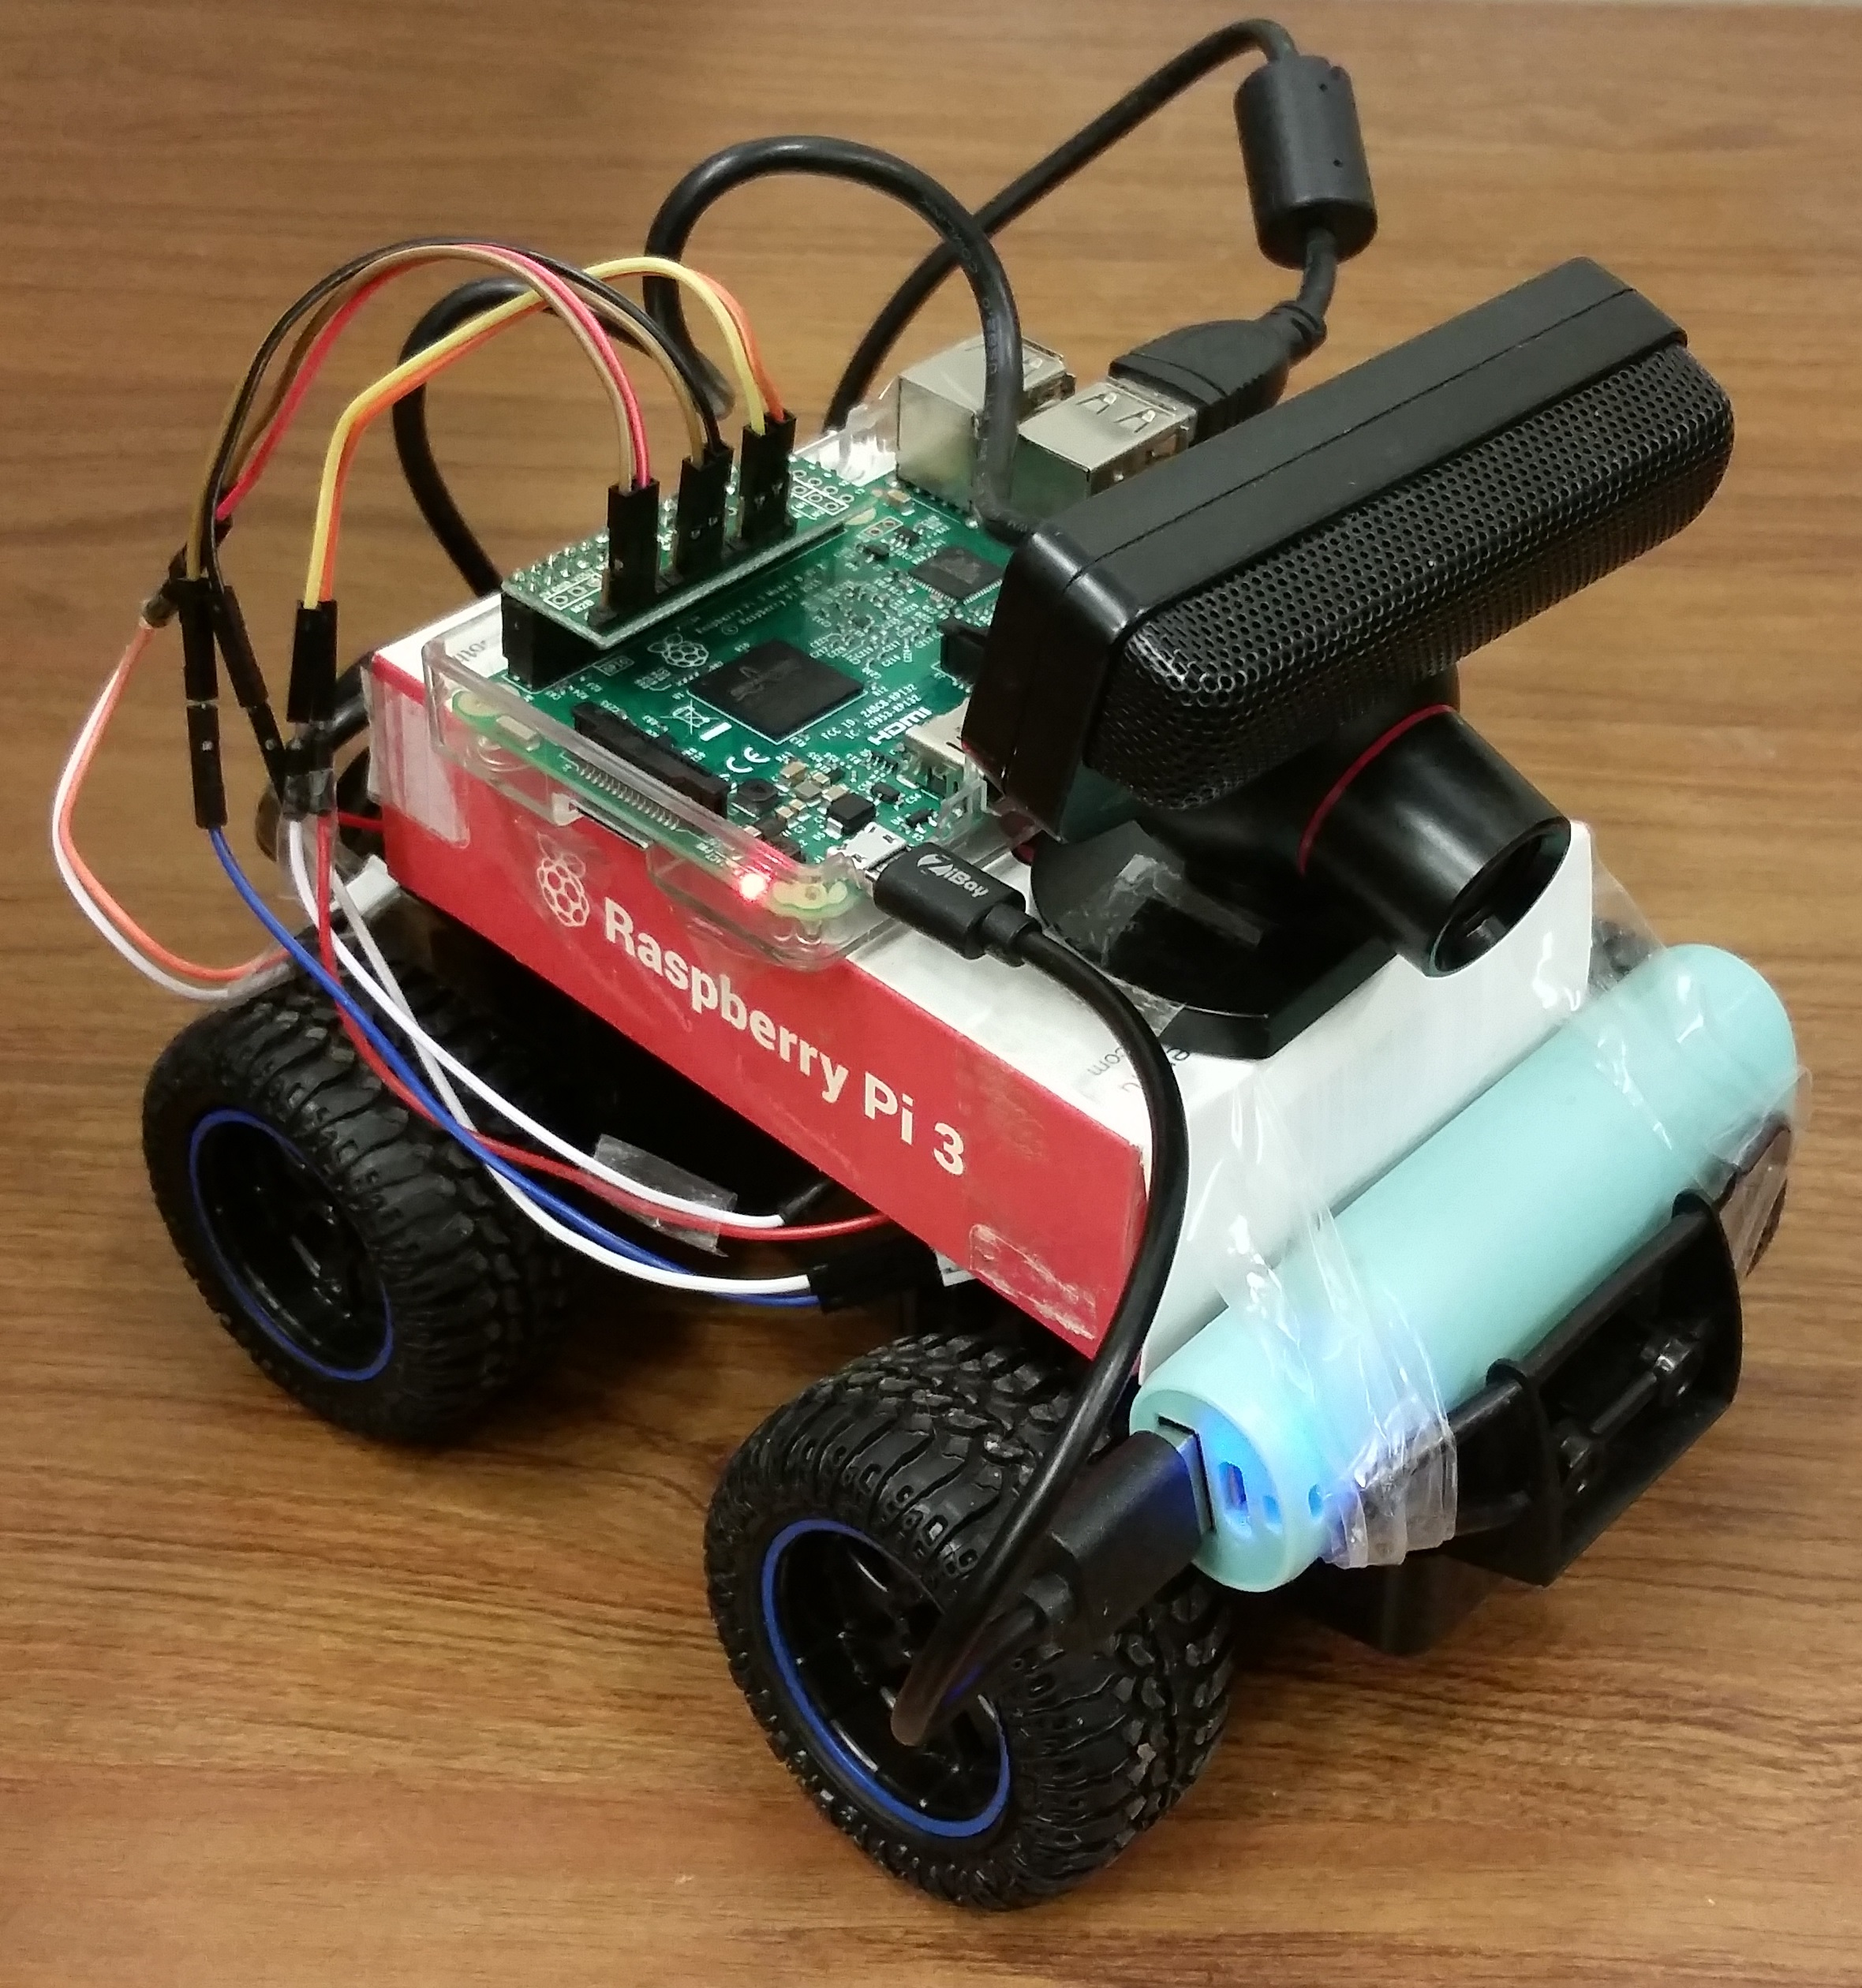
\includegraphics[width=.55\textwidth]{figs/DeepPicar_platform}
  \caption{DeepPicar platform.}
  \label{fig:overview}
\end{figure}

In this section, we provide an overview of our DeepPicar platform. In
developing DeepPicar, one of our primary goals is to replicate the
NVIDIA's DAVE-2 system on a smaller scale with using a low cost
multicore platform, the Raspberry Pi 3. Because the Pi 3's computing
performance is much lower than that of the DRIVE PX platform used in
DAVE-2, we are interested in if, and how, we can process
computationally expensive neural network operations in
real-time. Specifically, inferencing (forward pass processing)
operations must be completed within each control period
duration---e.g., a WCET of 33.$\overline{\mbox{33}}$ ms for 30Hz control 
frequency---locally on the Pi 3 platform, although training of the 
network (back-propagation for weight updates) can be done offline and 
remotely using a desktop computer.

Figure~\ref{fig:overview} shows the DeepPicar, which is comprised of a
set of inexpensive components: a Raspberry Pi 3 Single Board Computer
(SBC), a Pololu DRV8835 motor driver, a Playstation Eye webcam, a
battery, and a 1:24 scale RC car. Table~\ref{tbl:carbom} shows the
estimated cost of the system.

\begin{table}[t]
  \centering
  \begin{tabular}{|c|r|}
    \hline
    Item                    & Cost (\$) \\
    \hline
    Raspberry Pi 3 Model B  & 35 \\
    New Bright 1:24 scale RC car       & 10 \\
    Playstation Eye camera  &  7 \\
    Pololu DRV8835 motor hat&  8 \\
    External battery pack \& misc.   & 10 \\
    \hline
    Total                   & 70 \\
    \hline
  \end{tabular}
  \caption{DeepPicar's bill of materials (BOM)}
  \label{tbl:carbom}
\end{table}

For the neural network architecture, we adopt a TensorFlow version of
NVIDIA DAVE-2's convolutional neural network (CNN), published by Dr.
Fridman at  MIT~\footnote{https://github.com/lexfridman/deeptesla}. As
in DAVE-2, the CNN takes a raw color image (200x66 RGB pixels)
as input and produces a single steering angle value as
output. Figure~\ref{fig:architecture} shows the network architecture, which
is comprised of 8 layers, 250K parameters, and about 27 million
connections.

\begin{figure}[t]
  \centering
  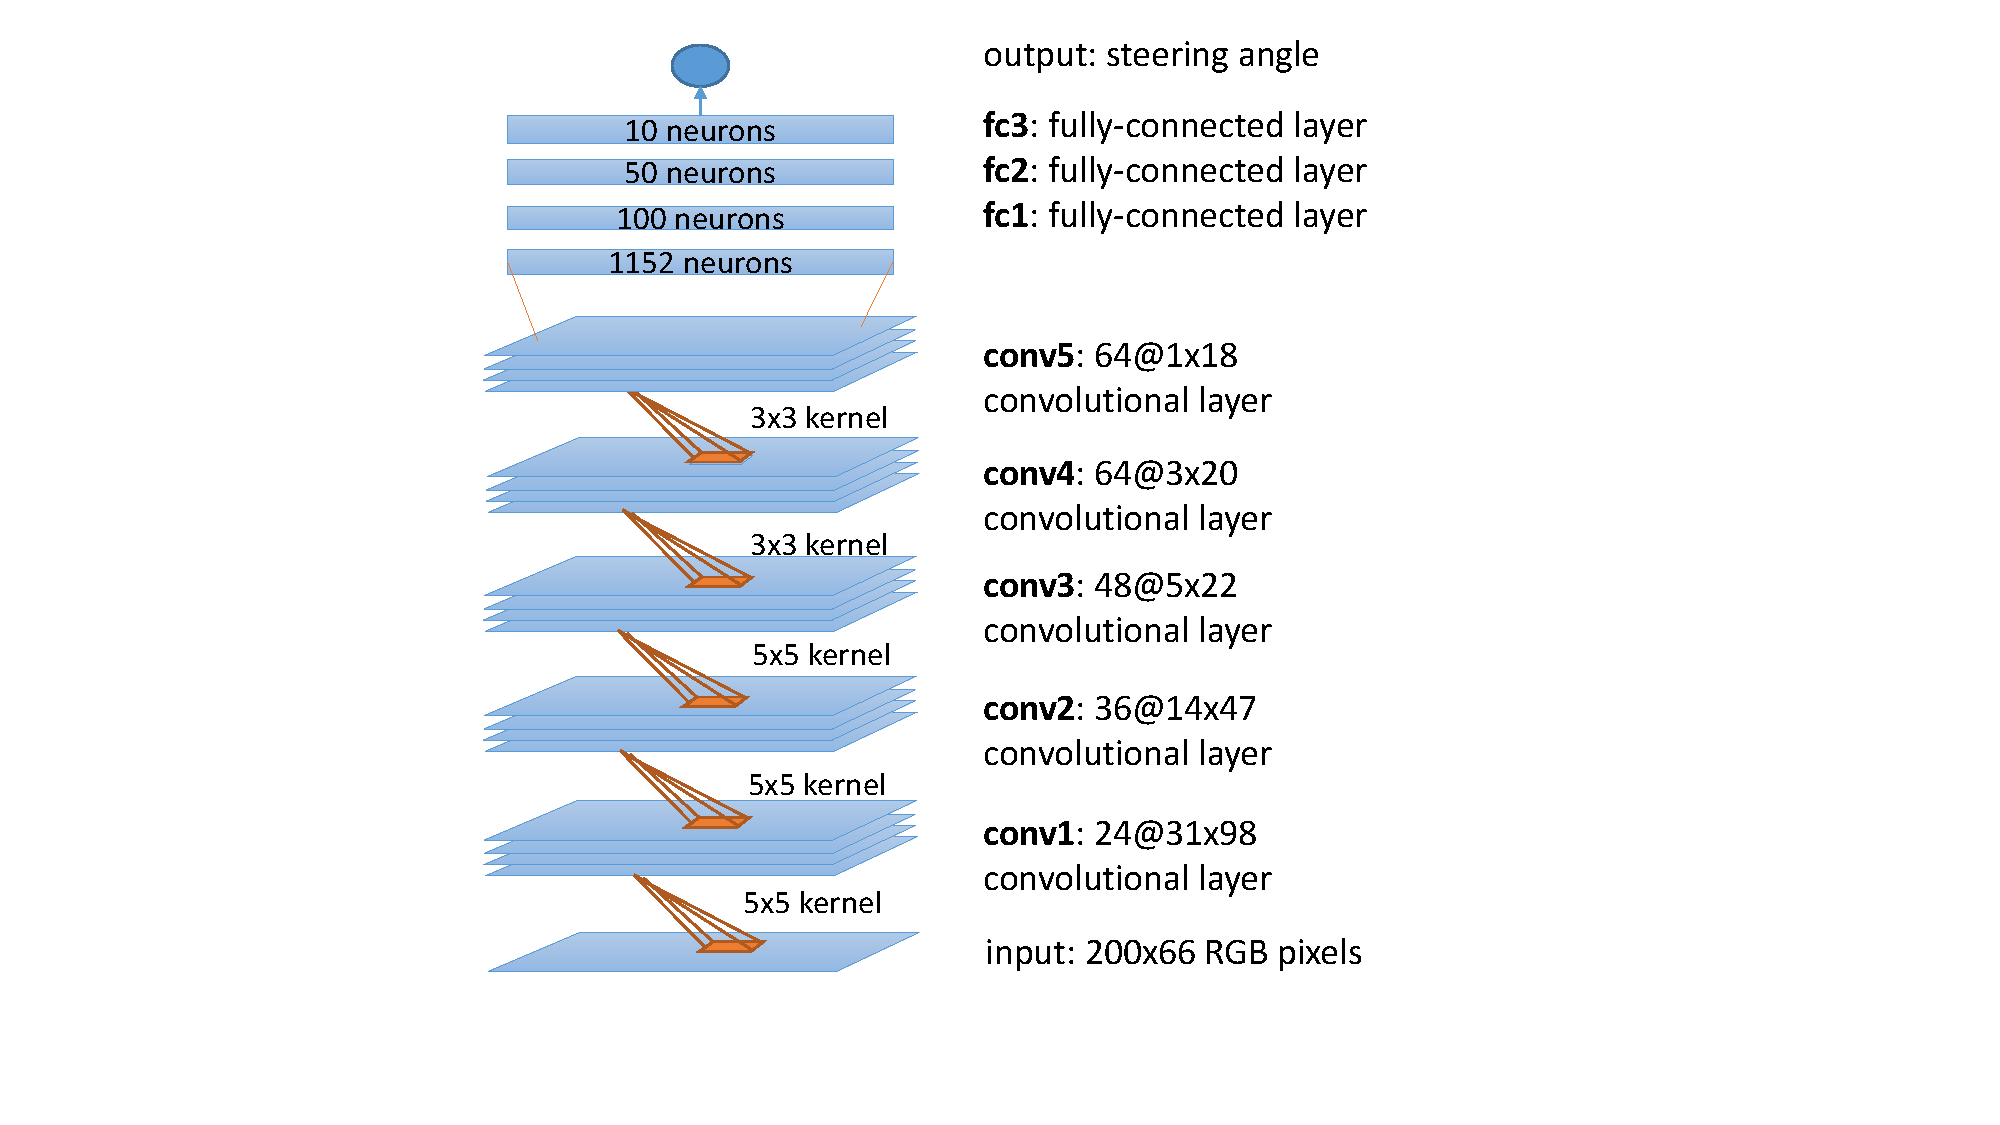
\includegraphics[width=\textwidth]{figs/architecture}
  \caption{DeepPicar's neural network architecture: 8 layers (5
    convolutional, 3 fully-connected layers), 27 million connections,
    250K parameters. The architecture is identical to the one used
    in NVIDIA's real self-driving car~\cite{Bojarski2016}.}
  \label{fig:architecture}
\end{figure}

\begin{figure}[t]
  \centering
  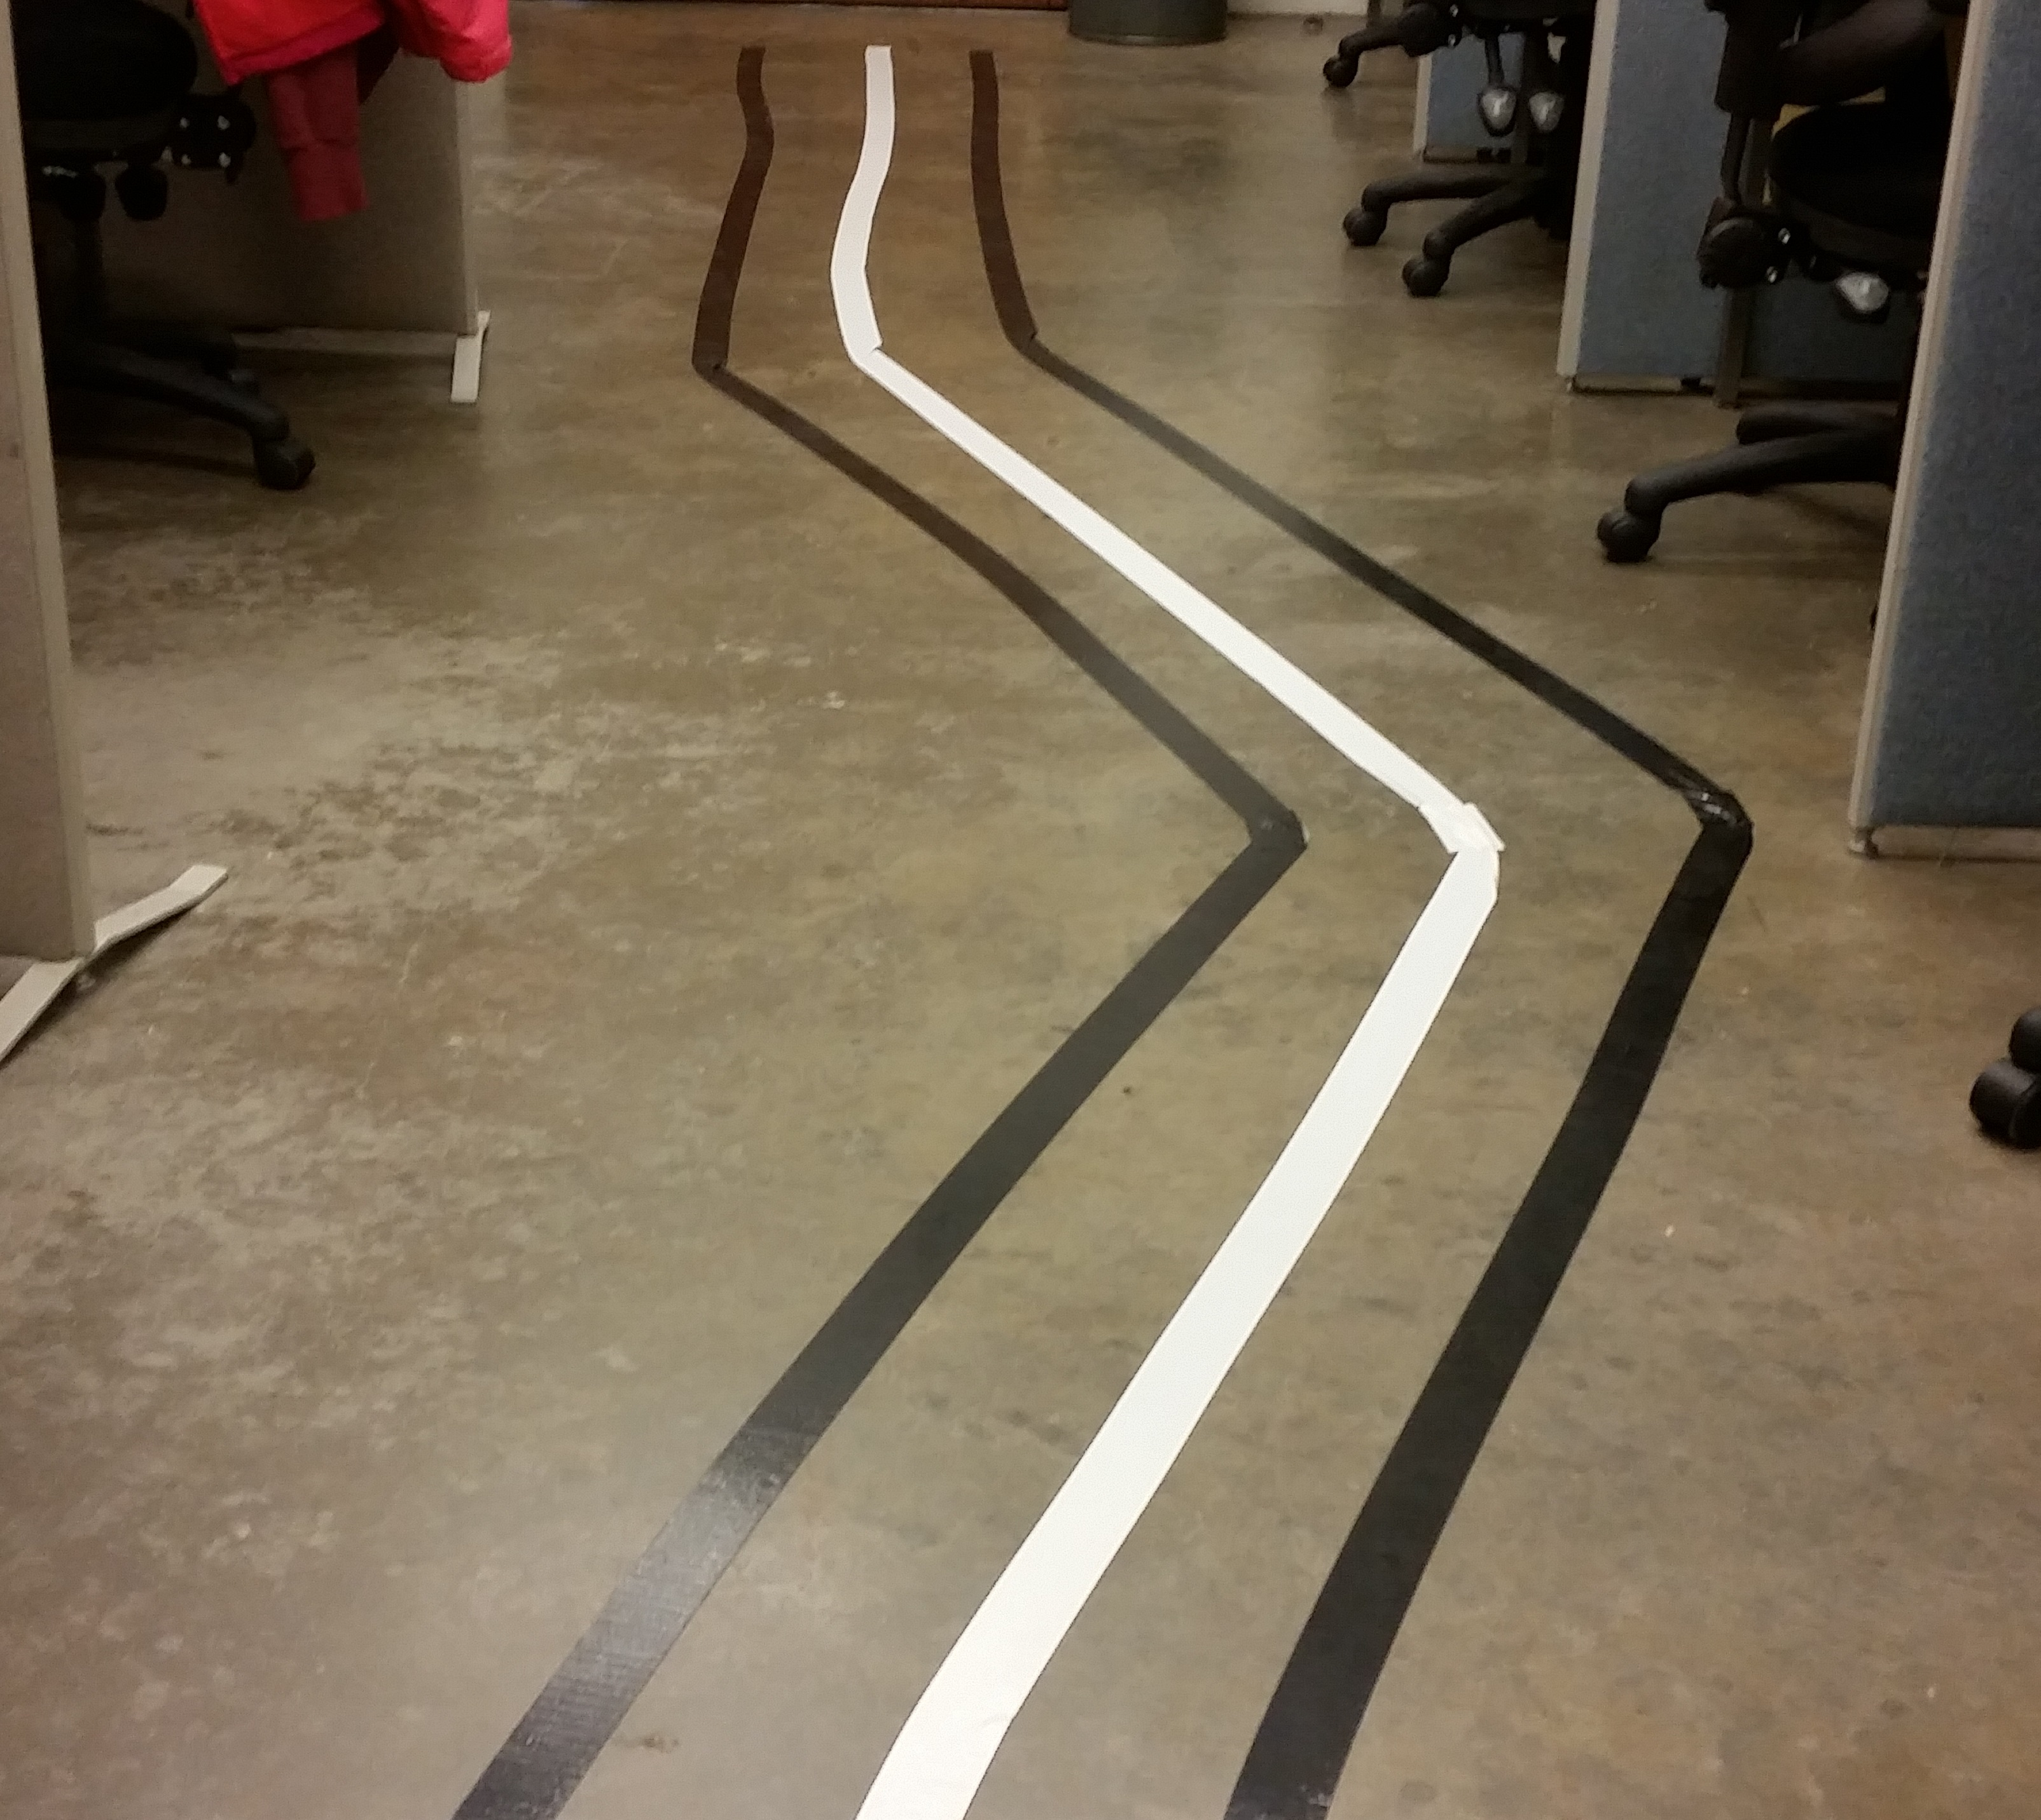
\includegraphics[width=.65\textwidth]{figs/track_new2}
  \caption{One of the custom tracks used for training/testing.}
  \label{fig:track}
\end{figure}

\begin{figure}[t]
   \lstset{language=python,
           basicstyle=\ttfamily\small,
           keywordstyle=\color{blue}\ttfamily,
           stringstyle=\color{red}\ttfamily,
           commentstyle=\color{green}\ttfamily
          }  
  \lstinputlisting[language=python]{control.py}
  \caption{Control loop}
  \label{fig:controlloop}
\end{figure}

% data collection and training.
To collect the training data, a human pilot manually drives the RC car
on a small track we created (Figure~\ref{fig:track}) to record
timestamped videos and contol commands. The stored data is then copied 
to a desktop computer, which is equipped with a NVIDIA GTX 1060 GPU, 
where we train the network to accelerate training speed. 
For comparison, training the network on the Raspbeery Pi 3 takes
approximately 4 hours, whereas it takes only about 5 minutes on the
desktop computer using the GTX 1060 GPU.

% inferencing on pi3
Once the network is trained on the desktop computer, the trained model
is copied back to the Raspberry Pi. The network is then used
by the car's main controller, which feeds a image frame from the web
camera as input to the network. In each control period, the produced 
steering angle output is then converted as the PWM values of the 
steering motor of the car. Figure~\ref{fig:controlloop} shows simplified 
pseudo code of the controller's main loop. Among the five steps, the 3rd step, 
network inferencing, is the most computationally intensive and dominates the
execution time.

Note that although the steering angle output of the network $angle$ is
a continuous real value, the RC car platform we used unfortunately
only supports three discrete angles---left (-30$^{\circ}$), center
(0$^{\circ}$), and right (+30$^{\circ}$)---as control inputs.
Currently, we approximate the network generated real-valued
angle to the closest one of the three angles, which may
introduce inaccuracy in control.
In the future, we plan to use a different (more expensive) RC car
platform that can precisely control the car's steering angle.
We would like to stress, however, that the use of different RC car
platforms has no impact on the computational 
aspects of the system, and that our main focus of this study is
not in improving network accuracy but in closely replicating the
DAVE-2's network architecture and its real-time characteristics.

Another issue we observed in training/testing the network, which could
affect the network performance, is camera latency. In DeepPicar's
context, the camera latency is from the time the camera
sensor observes the scene to the time the computer actually reads the
digitized image data. This time can be noticable depending on the camera 
used and the performance of the Pi. We experimentally measured the camera
latency and found it to be around 50-100 ms. This is higher than the 
latency of human perception, which is known to be as fast as 13 
ms~\cite{ThomasBurger2015}. Higher camera latency could negatively 
affect control performance, because the DNN would analyze stale scenes. 
In the future, we plan to identify and use low-latency cameras.

% https://www.pubnub.com/blog/2015-02-09-how-fast-is-realtime-human-perception-and-technology/

Despite these issues, the trained models were still able to
achieve a reasonable degree of accuracy, successfully navigating
several different tracks we trained. The source code, build
instruction, and a collection of self-driving videos of the DeepPicar
can be found at: \url{https://github.com/heechul/picar}.
